\documentclass[pdftex,12pt,letter]{article}
\usepackage{fancyhdr}
\usepackage{enumerate}
\usepackage{tabularx}
\usepackage{graphicx}
\usepackage{array}
\usepackage[toc,page]{appendix}
\usepackage[justification=justified,singlelinecheck=false]{caption}
\usepackage{placeins}
\pagestyle{fancy}
\makeatletter
  \renewcommand\@seccntformat[1]{\csname the#1\endcsname.\quad}
\makeatother

\newcolumntype {Y}{ >{\raggedright \arraybackslash }X}
\newcommand{\HRule}{\rule{\linewidth}{0.5mm}}
\captionsetup{labelformat=empty}

\begin{document}

\begin{titlepage}
\begin{flushright}
\HRule \\[0.4cm]
{ \bfseries
{\huge EECS 395 Project Proposal\\[1cm]}
{\Large for\\[1cm]}
{\huge Chocolate Box\large\\[.1cm]
A Procedural Level Generator for Unity\\[3cm]}
{\large Prepared by\\[1cm]James Fitzpatrick\\Stuart Long\\Frank Singel\\[2cm]
Version 1.0\\
February 3, 2014\\
}}
\end{flushright}
\end{titlepage}
\begin{table}[!h]
\caption*{\bfseries Revision History}
\begin{tabularx}{\textwidth }[t]{|l|l|Y|l|}
\hline
\bfseries Name & \bfseries Date & \bfseries Reasons for Change & \bfseries Version \\ \hline
\end{tabularx}
\end{table}
\FloatBarrier
\newpage
\section{Abstract}
\textit{Chocolate Box} will be a helpful tool for video game developers. Its goal is to provide an easy-to-use software library for any game developers working with the common game engine, Unity. It will allow developers to create unique levels purposed towards whatever game they are currently developing. These levels will be pseudo-random, so each level created will be unique. This tool will enable developers to create games with an infinite variety of levels which is perfect for arcade-like games. 
\\\\
\textit{Chocolate Box} will be built for 2-dimensional side-scrolling platformers, similar to classic games such as \textit{Super Mario Bros} and \textit{Megaman}. Users will be able to specify constraints and parameters on this library to mold the generated levels to fit their needs. 
\\\\
This system will be composed of a series of Unity scripts which users will interact with through the default Unity interface. The main issues involved in this project will be generating levels that are playable, fun, and fit developers' desires.
\newpage

\section{Introduction}
\subsection{Relevant Background}
Unity 4.3 was released a few short months ago in late 2013. One the major new features introduced was full support for 2D games. Before this new version, Unity had been intended as a game engined for 3D games, with any support for 2D having to come from unofficial and unsupported third parties. Given its recent introduction, there are currently not many libraries created for use with Unity's new 2D framework. Thus \textit{Chocolate Box} would be one of the first and it is certain that nothing like \textit{Chocolate Box} currently exists. Procedural level generation is both a challenging problem and a useful tool. In can be seen in modern games today such as \textit{Minecraft}, \textit{Terraria}, and \textit{Spelunky}. It allows games to provide an infinite variety of experiences for their players which keeps games interesting and long-lasting.
\subsection{Project Description}
\textit{Chocolate Box} will be a Unity asset that procedurally generates levels at runtime. Unity game developers will be able to incorporate this asset into their game scenes, allowing their games to have procedurally generated levels that smoothly integrate with their game's theme and the rest of their game. Procedurally generating a game level has many challenges associated with it. In brief, this problem encompasses determining a unique level layout and ensuring that layout is playable, fun, and constrains to user constraints. Users will use \textit{Chocolate Box} via a single Unity script. Therefore, they will interact with it via the Unity interface, specifically the Inspector.
\subsection{Related Work}
There currently does not exist any form of library to provide procedural level generation for Unity in either a 2D or 3D form. However, procedural level generation has been done for games such as \textit{Minecraft}. Such games are not open sourced and were not developed through Unity. 
\\\\
Two of the members of the \textit{Chocolate Box} team have experience with Unity. Stuart Long helped developed a fully functional game, \textit{Gumdrop Gauntlet}, in Unity. James Fitzpatrick has served as the design and programming leads for a number of Unity game demos, relevantly including a 2D puzzle-platformer, and a roleplaying game (RPG) in the style of Final Fantasy and Dragon Warrior. Frank Singel has the most experience on the team in the area of AI which will prove useful when creating the generation algorithms.
\subsection{Goals}
Below is described in detail the full feature set of \textit{Chocolate Box}, the team's methodology in developing it, and this project's software requirements. By the end of February, a month from now, the team expects to be able to generate a rudimentary level and to spawn enemies in it in a rudimentary fashion.

\section{Application}
\subsection{Environment Generation}
The first priority for the team is to create a functioning procedural environment generator. The environment will consist of the non-destructible areas upon which characters can move. This will also include the creation of dangerous terrain as well, such as spike traps, lava, and bottomless holes for the characters to fall through. The balance of walkable area and hazardous area will be determined by user parameters before the generation of each level. 
\\\\
Aside from the the Environment Generation will also create subsections of the overarching level structure. Each subsection will contain more harsh transtions between areas in the level. Examples of the division of subsections will include the alternation between inside and outside zones in a level or the alternation between a standard and lava filled cave. These subsections can be created by the user and will be generated at a parameterized rate as specified by the user. Each of these subsections will utilize transition areas between non-homogenous subsections. (Example: A transition between two outdoor areas will be noted by an open air area at the edge of the section. A transition from an outside to an inside area will be noted by a door with some evidence of a structure present). 
\\\\
Along with the interactible environments, the Environment Generation will also place non-essential elements to the background, such as trees. These elements, while not directly impacting gameplay, will add to the realism of level and, in a greater sense, the platformer. 
\\\\
Environment Generation will be lead by Stuart Long. Due to the importance of this task, Frank Singel will be assisting during the early stages of development.

\subsection{Enemy Generation}
The next highest priority for the team will be the randomized generation of enemies about the level. Based on the difficult parameter for the level specified, the level will have many or few enemies present. 
\\\\
Enemies will be of various forms and capabilities. There will be two types of enemies featured in our games: Ground and Aerial. 
\begin{itemize}

\item \textit{Ground Enemies}, as their names imply, will primarily be limited to Ground movement. In our generation,\textit{Ground Enemies} will be generated at the ground level, with a requisite amount of terrain as per the movement requirements of each. 

\item \textit{Aerial Enemies} are limited to airborn movement (at least initially). Aerial enemies will have a requiste aerial space for generation, primarily based on the movement pattern of the enemy. \\

\endgroup


Enemies will also have one of four different movement patterns: \textit{Stationary, Dumb, Intelligent, and Set}. Examples for this section will be taken from the \textit{Super Mario Bros.} Saga of video games. 
\begin{itemize}

\item \textit{Stationary Enemies} will not move from the spot of their creation. An example of a Stationary enemy is the \textit{Pirhanna Plant} from the \textit{Super Mario Bros.} saga of games.

\item \textit{Dumb Enemies} or \textit{Context Insensitive} will continuously move from their point of origin in a set direction without consideration of the environment around them. These enemies will stray and fall off cliffs or into other hazardous environments. An example of a Dumb Enemy is the \textit{Goomba} from the \textit{Super Mario Bros.} Saga of games.

\item \textit{Intelligent Enemies} or \textit{Context Sensitive} enemies will account for the existence of platforming perils and will move in such as way as to preserve their lives. An example of this enemy would be the \textit{Koopa Troopa}.

\item \textit{Set Enemies} will be limited to a unique pattern of movement. This is limited to a set area of movement as defined by further parameters set by the game developer. This area can be defined in the X, Y, or both dimensions. An example of this type of enemy would be \textit{The Hammer Bros.}\\

\endgroup

The movement patterns of each enemy will determine where each enemy can be appropriately placed, given the state of the environment. 
\\\\
Enemies, while maintaining many parameters, will also allow for the game developers to add custom scripts to have unique actions for each enemy. An example of this would be allowing enemies to have a number of hits taken before being destroyed. Scripted enemies can also take the players position into account through these scripts and act accordingly. Through these scripts, enemies can drop items that can benefit the player as per the Game Developer's design. 
\\\\
The Enemy Generation will be lead by James Fitzpatrick.

\subsection{Items Generation}
A constant feature in many games is the use of interactable items. These items serve many purposes and will appear at different frequencies. Example of items are listed below:
\begin{itemize}
\item \textit{Collectible Items} will be able to be picked up by the player over the course of a game. These items generally do not have an immediate benefit to the player and often have an effect on the players score at the end of levels. An example of this item is the \textit{Coin} or \textit{Ring} from \textit{Super Mario} and \textit{Sonic} franchises respectively. 

\item \textit{Power-Ups} are items that allow the player to enhance their capabilities. Examples of these items include \textit{Fire Flowers} from the \textit{Super Mario Bros}.

\item \textit{Interactible} items are able to be interacted with by the player and, logically, destroyed. These items are usually able to support player movement. Examples of these are the various blocks from the \textit{Super Mario} franchise. \\

\endgroup

Each item will have a set of parameters that will define its behavior. Some of these parameters will include but will not be limited to \textit{Frequency, Player Benefit, Difficulty to Acquire}. The exact function of each item will be defined by the Game Developer through Unity Scripts. 
\\\\
Item Generation will be lead by James Fitzpatrick

\subsection{Unity Platformer Game Demonstration}
To utilize all of the tools that we will be generating, there will be a playable demo game for the final presentation. The demo that will be created will take many of its influences from the \textit{Megaman} style of platformer.  Player interaction will be noted with a playable character that will have an array of weapons at the player's disposal. The platformer will utilize sectionalized environments with a variety of enemy types. 
\\\\
This demo will be designed during the last month of our development and will be led by Frank Singel with assistance from James Fitzpatrick and Stuart Long as necessary. 

\section{Methodology}
\subsection{Challenges}
\subsubsection{Flow}
One of the most important aspects of game design is the concept of \textit{flow}.  For the \textit{Chocolate Box} to be useful, it must ensure that games are sufficiently challenging, yet not too challenging as to keep players away from the game. While most of the  exact balancing of each level in the hands of the users, the library must enable the users to be able to adjust the difficulty of each level themselves in a meaningful way. Levels must have distinct differences between each other in terms of difficulty as well as other user modifiable parameters. 
\subsubsection{Performance}
For the \textit{Chocolate Box} to be a useful tool it must not be too large that it impacts the performance of the overall game. Utilizing algorithm optimization and by reducing the overal size of the necessary files, the generation algorithms will go unnoticed to the players. 
\subsubsection{Playability}
In the simplest sense, each game must generate playable levels. This problem is manyfold. Levels must be able to be completed from start to finish. Levels should also have limits on redundant level paths from start to finish. Dead ends, are also another dimension of video games, particularly in platformers, that should be reduced. These issues can all be addressed by effective and meaningful heursitics in level generation.
\subsubsection{Uniqueness}
Another challenge of procedural level generation is the idea of having a unique experience for each playthrough of the game. To compound this challenge, there must be some amount of consistency between levels such that there is a thematic unity to the game. Further, there must be a uniqueness between sections of each level. Having a varied structure to each level will increase playback rates as well as improve overall user experience. By defining appropriate heuristics and parameters for user modificiation, the library will allow for such variety. 
\subsubsection{Usability}
One of the largest challenges for this project is for the \textit{Chocolate Box} to not just be powerful, but also easy to use. There are many powerful tools at the disposal of users. Often these tools are too feature heavy and less important tools can convolute the strengths of many features of similar libraries. The library tool be too complex that it cannot allow for a quickened game design workflow. It also must be able to seemlessly adapt to a variety of user assets. By using many built-in WYSIWYG features of Unity, this challenge will be simplified. 


\section{Software Design}
\subsection{User Classes}
Our users will be varying types of game developers. These users will range from individuals looking to make games recreationally, to groups doing game design projects. The type of games that users will be developing with this API will typically be side-scrolling shooters and platforming games. Such games often feature enemy units of varying types.
\subsection{Operating Environment}
This library will be designed to work with Unity 4.3 and newer. Scripts will be written in C\#, based on Unity's native support of it.
\subsection{Performance Constraints}
This library will procedurally generate a playable, pseudo-random level in under 30 seconds. This level will vary depending on user-defined parameters, such as difficulty and size. We will keep the file size under 50MB.
\subsection{Software Specifications}
This project will be completed as one manager script that will call upon many background scripts. Some of the background script functions will include: platform generation, level playability testing, enemy placement, and object placement.
\subsection{Data Structures}
Our library will take advantage of Unity's cohesive interfaces to allow users to seemlessly incorporate their assets. As a result, many of our structures will inheirit from  Unity native objects. Some of the internal data structures we will use will include a base “enemy” class, from which we will base different types of enemy spawn locations based on what types of enemies (such as flying, walking, and stationary) they are. We will also include a class for collectables, which will encompass various pickups such as health, ammo, coins, etc. Also, by using GameObjects as storage points for user content, we will be able to use Unity's drag-and-drop functionality to navigate and expand our generator's functionalities and use additional assets in level creation.
/subsection{Software Architecture}
This will be a library to be included in Unity 4.3 projects.

\section{Project Management}
The \textit{Chocolate Box} team is small and familiar, allowing for a more project management schema. Stuart Long is the project manager and he will be responsible for the overall project management. Each member of the team will have set responsibilities, but the team as a whole will collaborate on any challenges or problems that arise if need be. The team will be using the on-line task tracking system Trello to keep track of project tasks and bugs. A private git repository on GitHub has been secured to use as the version control system for the project. Below is a Gantt chart outlining the broad goals and time-line of the project that the team have so far determined.
\centerline{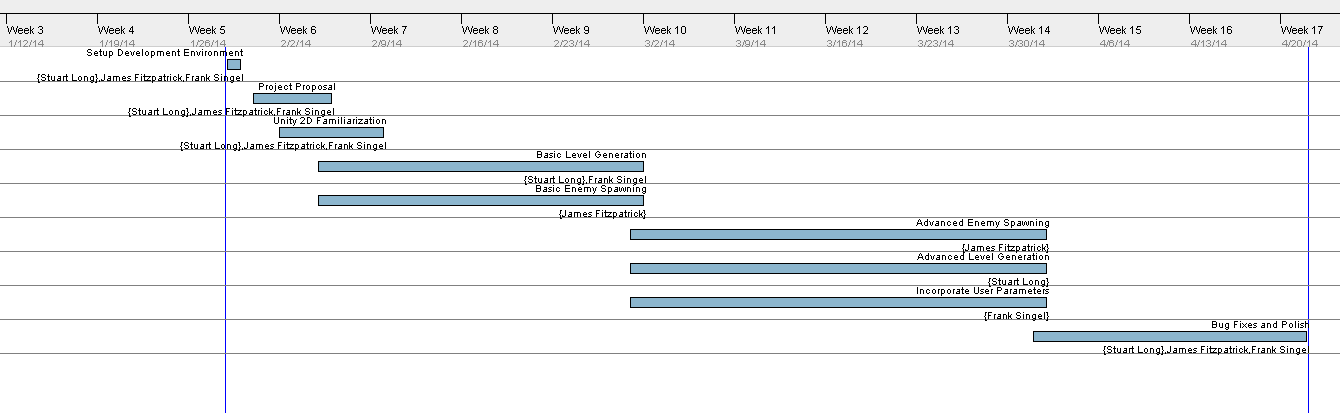
\includegraphics[width=7in]{GanttSS.png}}
\FloatBarrier
\section{User Interface}
\textit{Chocolate Box} will be fully integrated into Unity. Thus it will not requires its own User Interface. Instead, it will be used through Unity's own interface, specifically the part known as the Inspector. A mock up of this interface can be seen on the right-hand side of the figure below.

\centerline{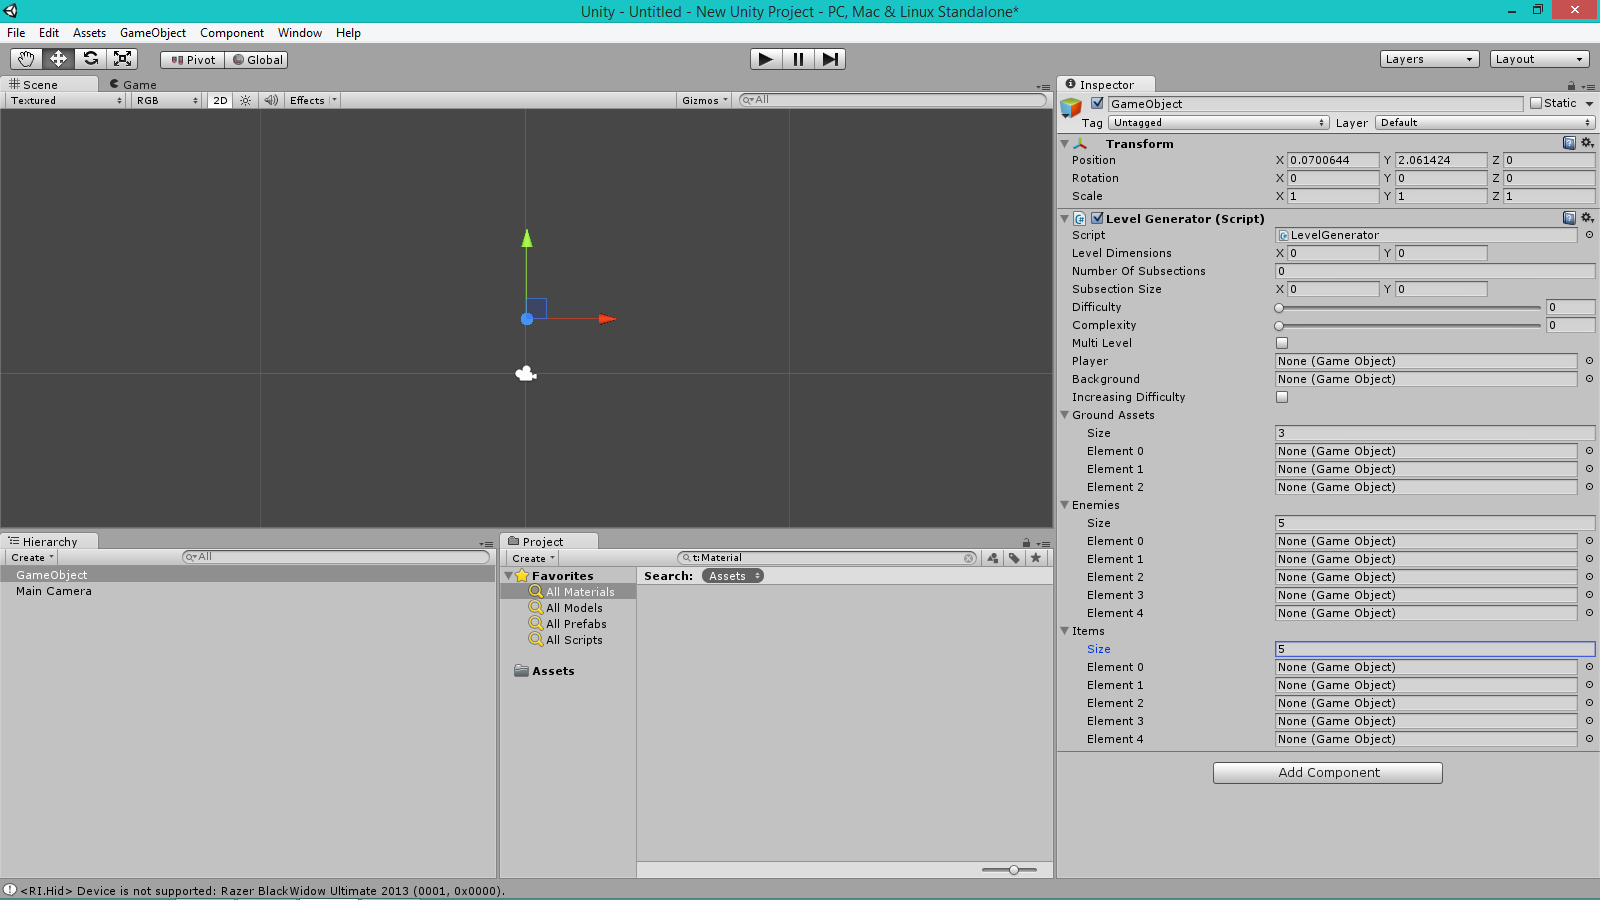
\includegraphics[width=7in]{UnitySS.png}}
\FloatBarrier
\end{document}